\documentclass[aspectratio=169]{beamer}
\usepackage{will_handley_beamer}
\usepackage{title_page}

% Commands
% --------
% - \arxiv{arxiv number}
% - \cols{width}{lh column}{rh column}
% -  \begin{fig(left|right)}[fractional width (e.g 0.6) ]{name of image}
%        content of other column
%    \end{fig(left|right)}

% Talk details
% ------------
\title{<+Title+>}
\subtitle{<+subtitle+>}
\date{<+Date+>}

\begin{document}

\begin{frame}
    \titlepage
\end{frame}

\begin{frame}
    \frametitle{<+Bayesian slide+>}
    \begin{itemize}
        \item Bayes theorem
        \item Joint
    \end{itemize}<++>
\end{frame}

\begin{frame}
    \frametitle{Applications: The three pillars of Bayesian inference}
    \begin{columns}[t]
        \column{0.33\textwidth}
        \begin{block}{Parameter estimation}
            What do the data tell us about the parameters of a model?

            \textit{e.g. the size or age of a $\Lambda$CDM universe}
            \[ \hspace{-4pt}\C[0]{P(\theta|D,M)} = \frac{\C[2]{P(D|\theta,M)} \C[1]{P(\theta|M)}}{\C[3]{P(D|M)}} \] 
            \[ \C[0]{\mathcal{P}} = \frac{\C[2]{\mathcal{L}} \times\C[1]{\pi}}{\C[3]{\mathcal{Z}}}\] 
            \[ \C[0]{\text{Posterior}} = \frac{\C[2]{\text{Likelihood}} \times\C[1]{\text{Prior}}}{\C[3]{\text{Evidence}}}\]
        \end{block}
        \column{0.3\textwidth}
        \begin{block}{Model comparison}
            How much does the data support a particular model?

            \textit{e.g. $\Lambda$CDM vs a dynamic dark energy cosmology}
            \[ \C[4]{P(M|D)} = \frac{\C[3]{P(D|M)} \C[5]{P(M)}}{\C[7]{P(D)}} \vspace{-7pt}\]
            \[ \frac{\C[3]{\mathcal{Z}_\mathcal{M}} \C[5]{\Pi_\mathcal{M}}}{\C[7]{\sum_m Z_m \Pi_m}} \]
            \[ \C[4]{\text{Posterior}} = \frac{\C[3]{\text{Evidence}} \times\C[5]{\text{Prior}}}{\C[7]{\text{Normalisation}}}\]
        \end{block}
        \column{0.33\textwidth}
        \begin{block}{Tension quantification}
            Do different datasets make consistent predictions from the same model? 
            \textit{e.g. CMB vs Type IA supernovae data}
            \[ \mathcal{R} = \frac{\C[3]{\mathcal{Z}}_{AB}}{\C[3]{\mathcal{Z}}_A\C[3]{\mathcal{Z}}_\mathcal{B}}\] 
            \[
                \begin{aligned} \log\mathcal{S} = \av[{\C[0]{\mathcal{P}}_{AB}}]{\C[2]{\log\mathcal{L}}_{AB}}&\\
                    -\av[{\C[0]{\mathcal{P}}_{A}}]{\C[2]{\log\mathcal{L}}_{A}}&\\
                    -\av[{\C[0]{\mathcal{P}}_{B}}]{\C[2]{\log\mathcal{L}}_{B}}&
                \end{aligned}
            \]
        \end{block}
    \end{columns}
\end{frame}

\begin{frame}
    \frametitle{Conclusions}
    \framesubtitle{\href{https://www.github.com/handley-lab}{github.com/handley-lab}}
    \tikz[overlay,remember picture]
        \node[anchor=north east] (A) at ($(current page.north east)+(0,0)$) {
            
\includegraphics[width=0.09\textheight]{figures/students/adam_ormondroyd.jpg}%
            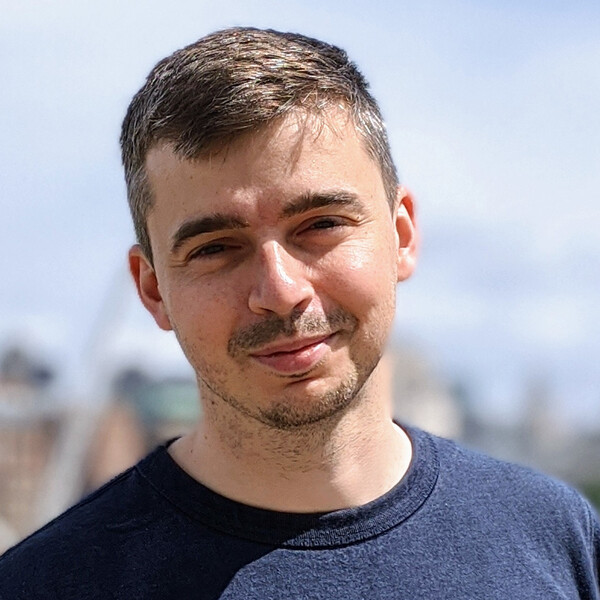
\includegraphics[width=0.09\textheight]{figures/students/david_yallup.jpg}%
            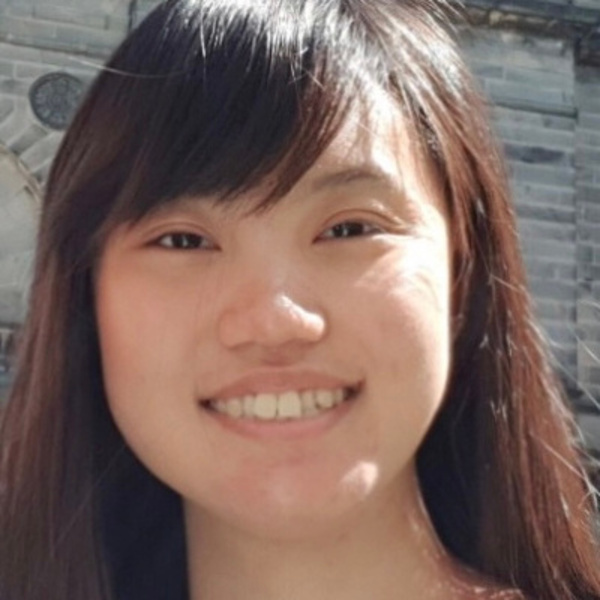
\includegraphics[width=0.09\textheight]{figures/students/dily_ong.jpg}%
            
\includegraphics[width=0.09\textheight]{figures/students/felicity_ibrahim.jpg}%
            
\includegraphics[width=0.09\textheight]{figures/students/george_carter.jpg}%
            
\includegraphics[width=0.09\textheight]{figures/students/harry_bevins.jpg}%
            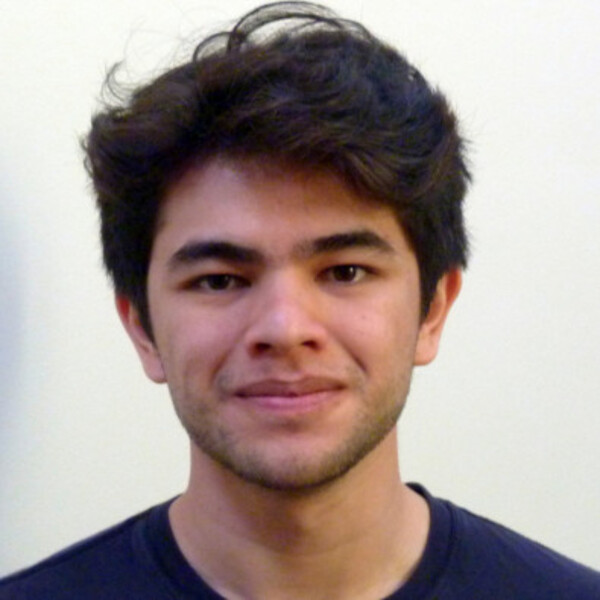
\includegraphics[width=0.09\textheight]{figures/students/ian_roque.jpg}%
            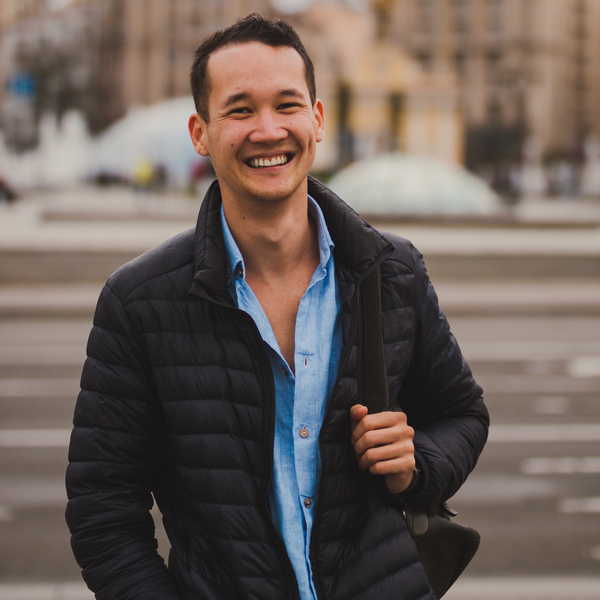
\includegraphics[width=0.09\textheight]{figures/students/kilian_scheutwinkel.jpg}%
            
\includegraphics[width=0.09\textheight]{figures/students/metha_prathaban.jpg}%
            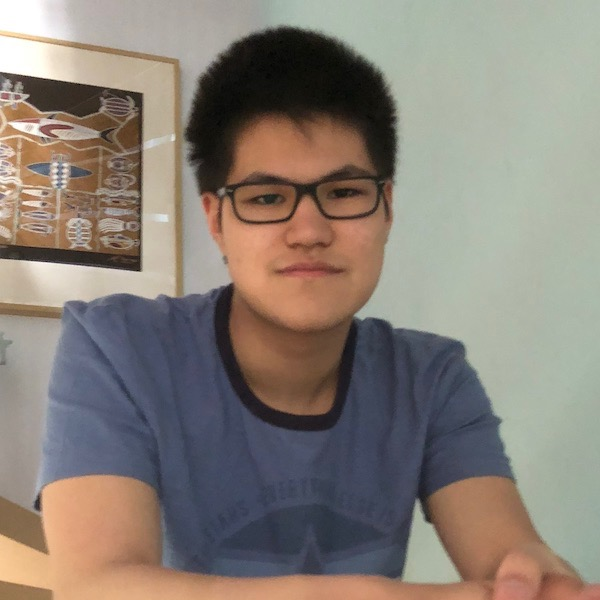
\includegraphics[width=0.09\textheight]{figures/students/namu_kroupa.jpg}%
            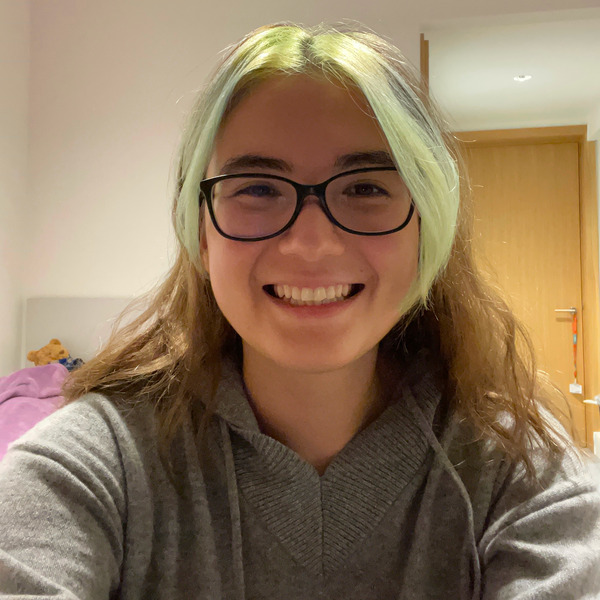
\includegraphics[width=0.09\textheight]{figures/students/sinah_legner.jpg}%
            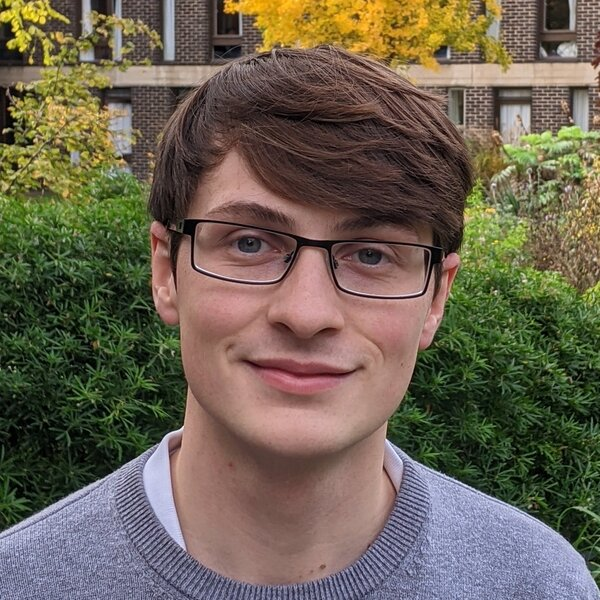
\includegraphics[width=0.09\textheight]{figures/students/thomas_gessey-jones.jpg}%
            
\includegraphics[width=0.09\textheight]{figures/students/tze_goh.jpg}%
            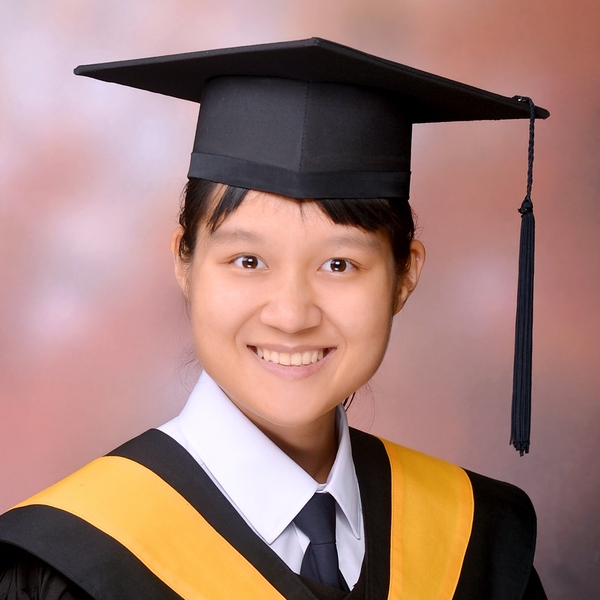
\includegraphics[width=0.09\textheight]{figures/students/wei-ning_deng.jpg}%
    };
\end{frame}

\end{document}
